\documentclass[11pt,letterpaper]{article}
\usepackage[utf8]{inputenc}
\usepackage[spanish]{babel}
\usepackage{csquotes} % recomendation of biblatex alongside babel
\usepackage{amsmath}
\usepackage{amsfonts}
\usepackage{amssymb}
\usepackage{graphicx}
\usepackage{subcaption}
\usepackage[left=2cm,right=2cm,top=2cm,bottom=2cm]{geometry}
\usepackage{hyperref}
\hypersetup
{
    colorlinks=true,
    citecolor=blue,
    linkcolor=blue,
    filecolor=blue,      
    urlcolor=blue,
    pdfstartview={FitH}
}

% For directory draw
\usepackage{fancyvrb}
\usepackage[T1]{fontenc}
\usepackage{pmboxdraw}
\usepackage{newunicodechar}
\newunicodechar{└}{\textSFii}
\newunicodechar{├}{\textSFviii}
\newunicodechar{─}{\textSFx}

\author
{
	Camilo Ocampo\\
 	{\tt miloog@gmail.com}
}
\title{\bf MAPA INTERACTIVO PARA LA IDENTIFICACIÓN DE LAS PROBLEMÁTICAS AMBIENTALES EN EL MUNICIPIO DE MEDELLÍN}
\date{Diciembre 2016}

\begin{document}
\maketitle

\section{Introducción}
El mapa interactivo aquí documentado representa un producto enfocado y minimo viable para mostrar información relevante de las problemáticas ambientales en el municipio de Medellín. Se seleccionó el desarrollo web como plataforma para el aplicativo dada su versatilidad a la hora de compartir la información tanto {\it online} como {\it offline}. Para su desarrollo se adoptó la filosofía {\it mobil first} que orienta el diseño hacia una plataforma responsive. Las herramientas fundamentales usadas para el desarrollo fueron HTML5, CSS3 y Javascript. Con el objetivo de mejorar la velocidad y eficiencia en el desarrollo se incluyeron dentro del entorno de desarrollo: El sistema de control de versiones Git \cite{git}, los administradores de paquetes npm \cite{npm} y Bower \cite{bower}, y el ejecutador de tareas Gulp \cite{gulp}. Finalmente se apoyó el diseño e interactividad de la plataforma haciendo uso de los {\it frameworks}: Bootstrap \cite{bootstrap}, jQuery y Leaflet \cite{leaflet}.
\vspace{1cm}
\begin{figure}[ht]
\centering
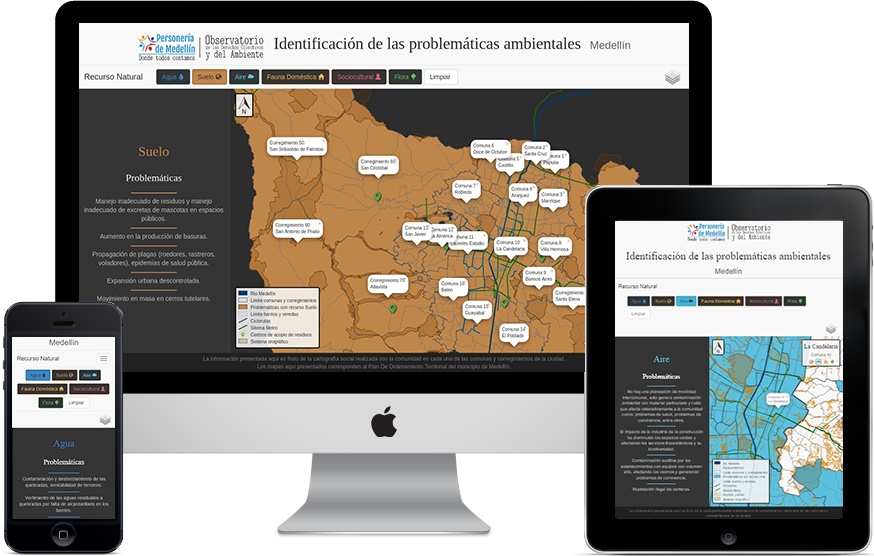
\includegraphics[width=0.7\textwidth]{../assets/images/responsive.png}
\caption{Demostración de diseño responsive. Esta imagen puede encontrarse en:\\ {\tt assets/images/responsive.png}}\label{fig:responsive}
\end{figure}

\section{Distribución del proyecto}

\subsection{Directorio raíz}
El directorio raíz del proyecto se muestra en la figura \ref{fig:root}. Los archivos fuente de la aplicación se encuentran en el directorio {\tt app}. La documentación, su fuente en \LaTeX\ y este documento pueden encontrarse en el directorio {\tt doc}. El directorio dist es generado automaticamente al compilar el proyecto y contiene los archivos necesarios para compartir la plataforma online u offline segun la configuración. 

\begin{figure}[ht]
\centering
\begin{BVerbatim}
mdlln-map
├── app
├── assets
├── bower_components
├── bower.json
├── dist
├── doc
├── gulpfile.js
├── node_modules
├── package.json
├── README.md
└── test
\end{BVerbatim}
\caption{Raíz del proyecto.}\label{fig:root}
\end{figure}

Los archivos: {\tt bower.json}, {\tt gulpfile.js} y {\tt package.json} corresponden a los archivos de configuración del entorno de desarrollo y los administradores de paquetes. Estos son los encargados de generar los directorios {\tt bower\_components}, {\tt dist}, {\tt node\_modules} y {\tt test}. Se recomienda prudencia al modificarlos, Los directorios {\tt bower\_components} y {\tt node\_modules} algunas dependencias fundamentales para la compilación del proyecto.

Finalmente el archivo {\tt README.md}, contiene una guia para configurar un entorno de desarrollo en formato markdown.

\subsection{Codigo fuente del aplicativo}

En el directorio {\tt app} se encuentran los archivos fuente del aplicativo. La estructura del directorio se puede apreciar en la figura \ref{fig:app}. Se destacan en este directorio los archivos {\tt index.html}, {\tt main.js} y {\tt main.scss}. El aplicativo recide fundamentalmente en estos tres archivos, donde el primero contiene la estructura del contenido, el segundo las funciones y declaraciones de Javascript necesarias para su interactividad y el tercero la información de los estilos para el contenido. Este ultimo en formato SASS \cite{sass} que posteriormente será compilado en un archivo CSS.

\begin{figure}[ht!]
\centering
\begin{BVerbatim}
app
├── favicon.ico
├── index.html
├── robots.txt
├── scripts
│   ├── comcorr.js
│   ├── leaflet-src.js
│   ├── main.js
│   └── resources.js
├── styles
│   ├── images
│   ├── leaflet.css
│   └── main.scss
├── support_maps
└── tutorial
\end{BVerbatim}
\caption{Código fuente del aplicativo.}\label{fig:app}
\end{figure}

Los archivos {\tt leaflet-src.js} y {\tt leaflet.css} corresponden al framework para mapas interactivos Leaflet.

En el directorio {\tt support\_maps} se encuentra la información de los mapas en formato geoJson (Formato popular para contenido cartográfico en la web.). 

En el directorio {\tt tutorial} se encuentran las imagenes {\tt .gif} mostradas en el manual de usuario del aplicativo.

Los archivos dentro de la carpeta {\tt app/styles/images/} son necesarios para la correcta presentación de la información. Entre estos se encuentran los logos institucionales, etc.

\subsection{Activos del proyecto}

En la capeta {\tt assets} del directorio raíz pueden encontrarse los mapas originales usados para el proyecto en diferentes formatos ({\tt raw\_maps.zip}), así como imagenes e impresiones de pantalla del aplicativo final ({\tt assets/images/}). Cómo se mencionó antes, los mapas en formato geoJson pueden ser encontrados en {\tt app/support\_maps/} y las imagenes animadas mostradas en el manual de usuario en {\tt app/tutorial/}.

\begin{figure}[ht!]
\centering
\begin{subfigure}{.49\textwidth}
	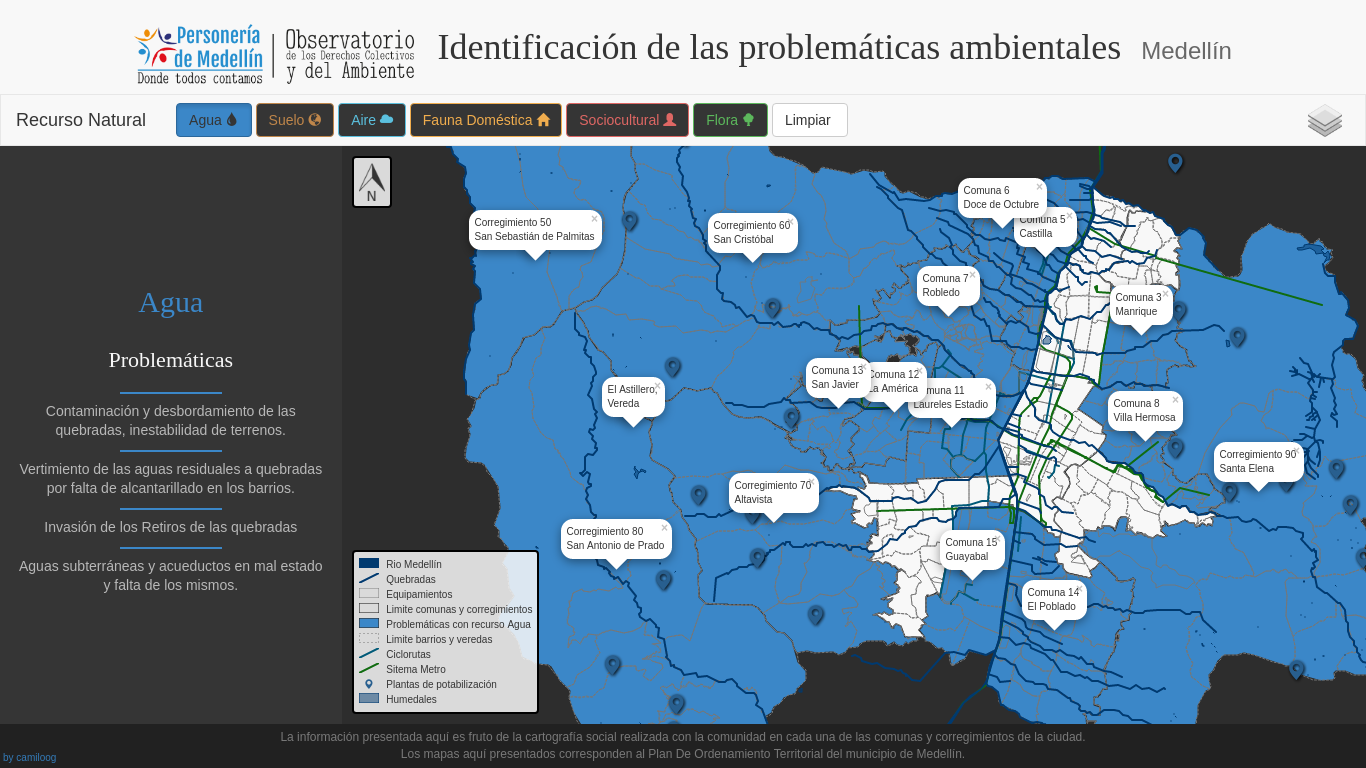
\includegraphics[width=\textwidth]{../assets/images/recurso_natural/recurso_agua.png}
	\caption{Agua}\label{fig:rAgua}
\end{subfigure}	
\hfill
\begin{subfigure}{.49\textwidth}
	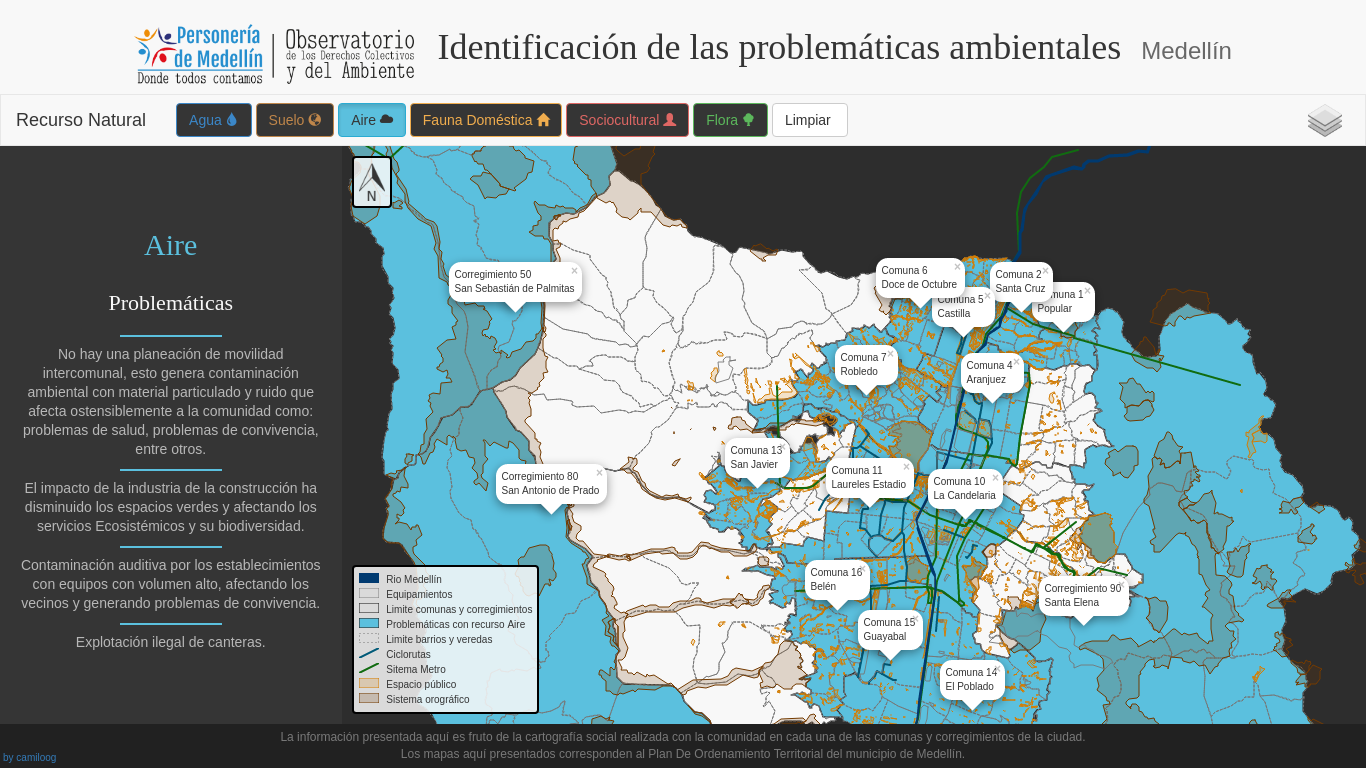
\includegraphics[width=\textwidth]{../assets/images/recurso_natural/recurso_aire.png}
	\caption{Aire}\label{fig:rAire}
\end{subfigure}

\begin{subfigure}{.49\textwidth}
	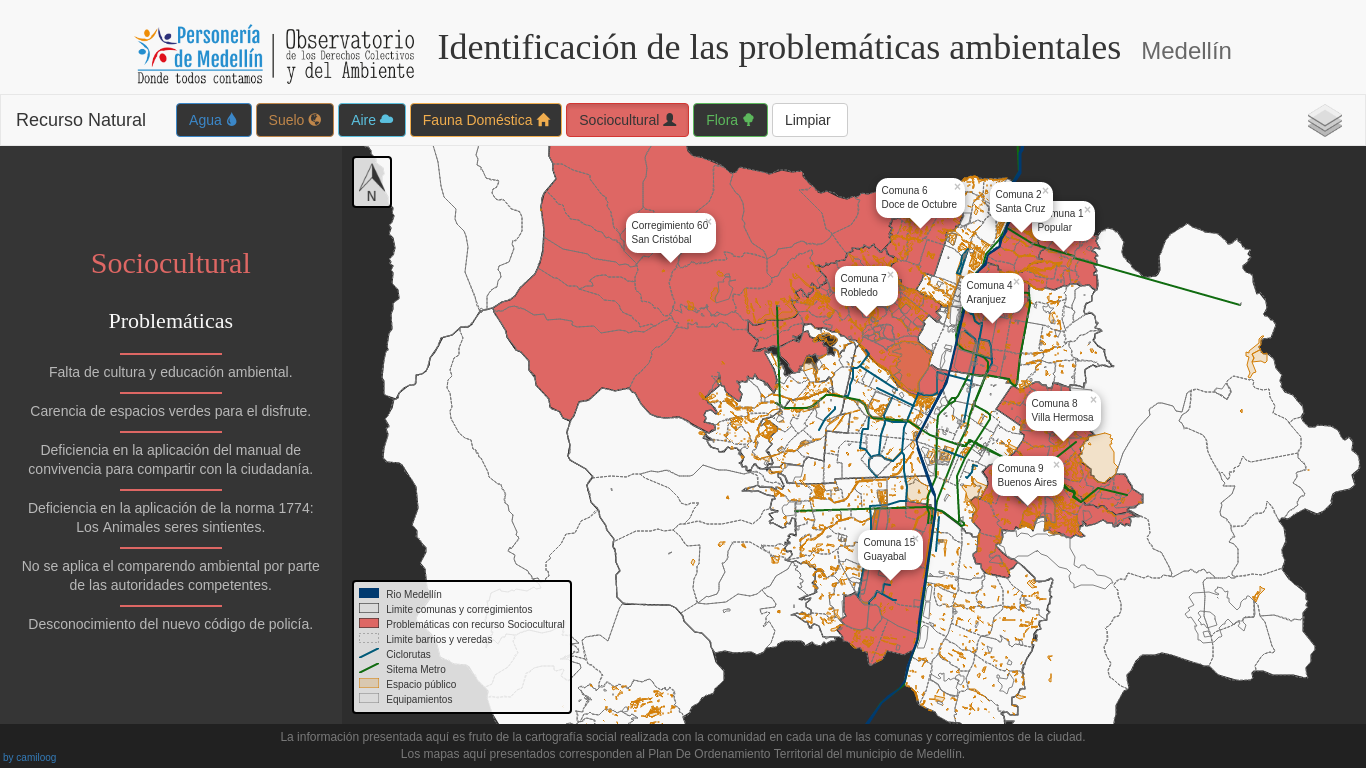
\includegraphics[width=\textwidth]{../assets/images/recurso_natural/recurso_sociocultural.png}
	\caption{Sociocultural}\label{fig:rSociocultural}
\end{subfigure}	
\hfill
\begin{subfigure}{.49\textwidth}
	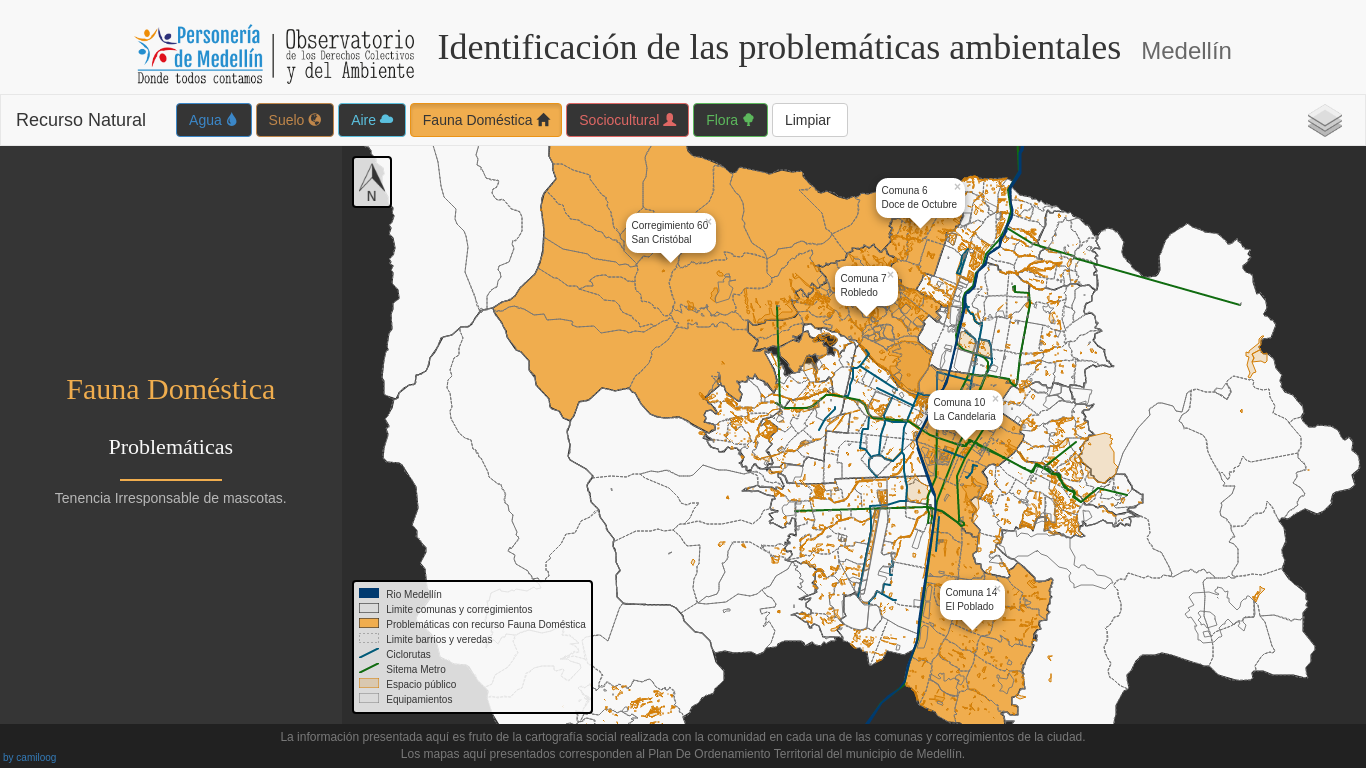
\includegraphics[width=\textwidth]{../assets/images/recurso_natural/recurso_fauna_domestica.png}
	\caption{Fauna doméstica}\label{fig:rFauna}
\end{subfigure}				

\begin{subfigure}{.49\textwidth}
	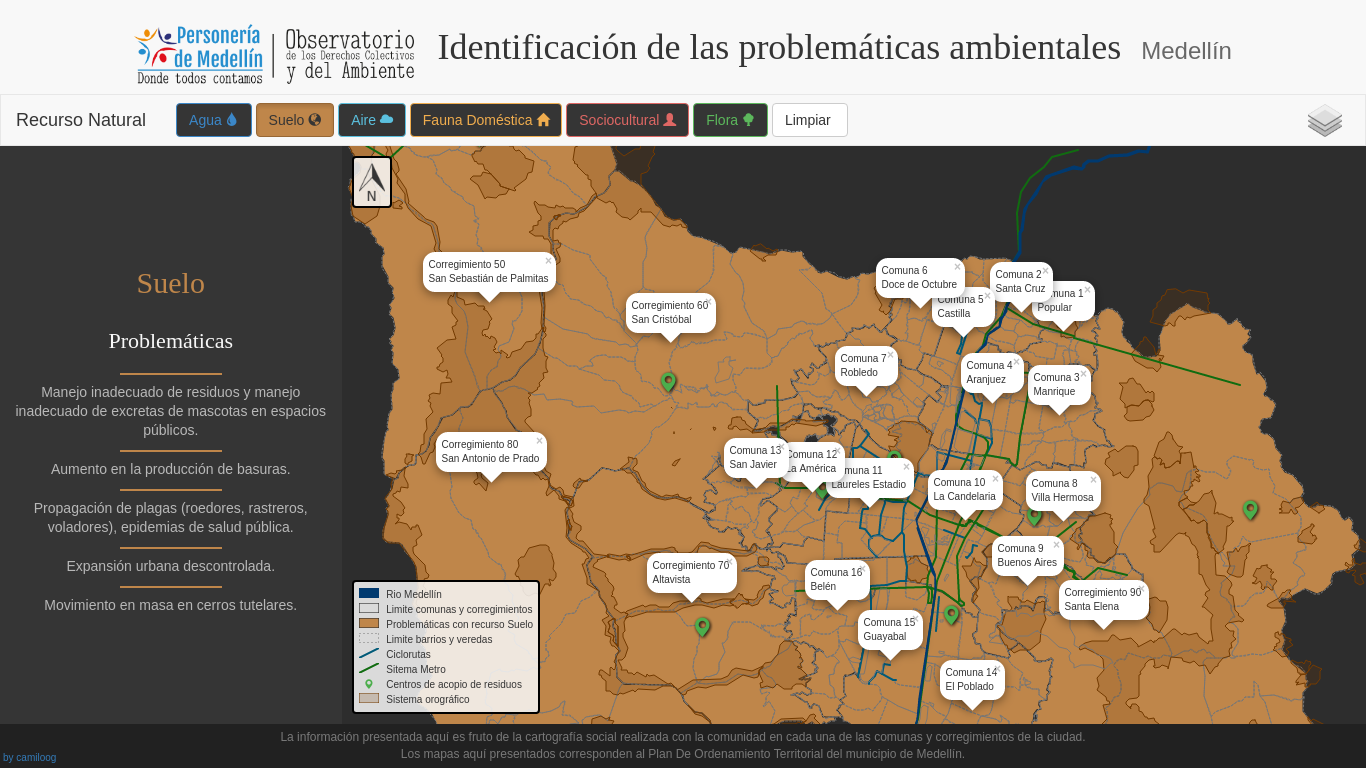
\includegraphics[width=\textwidth]{../assets/images/recurso_natural/recurso_suelo.png}
	\caption{Suelo}\label{fig:rSuelo}
\end{subfigure}	
\hfill
\begin{subfigure}{.49\textwidth}
	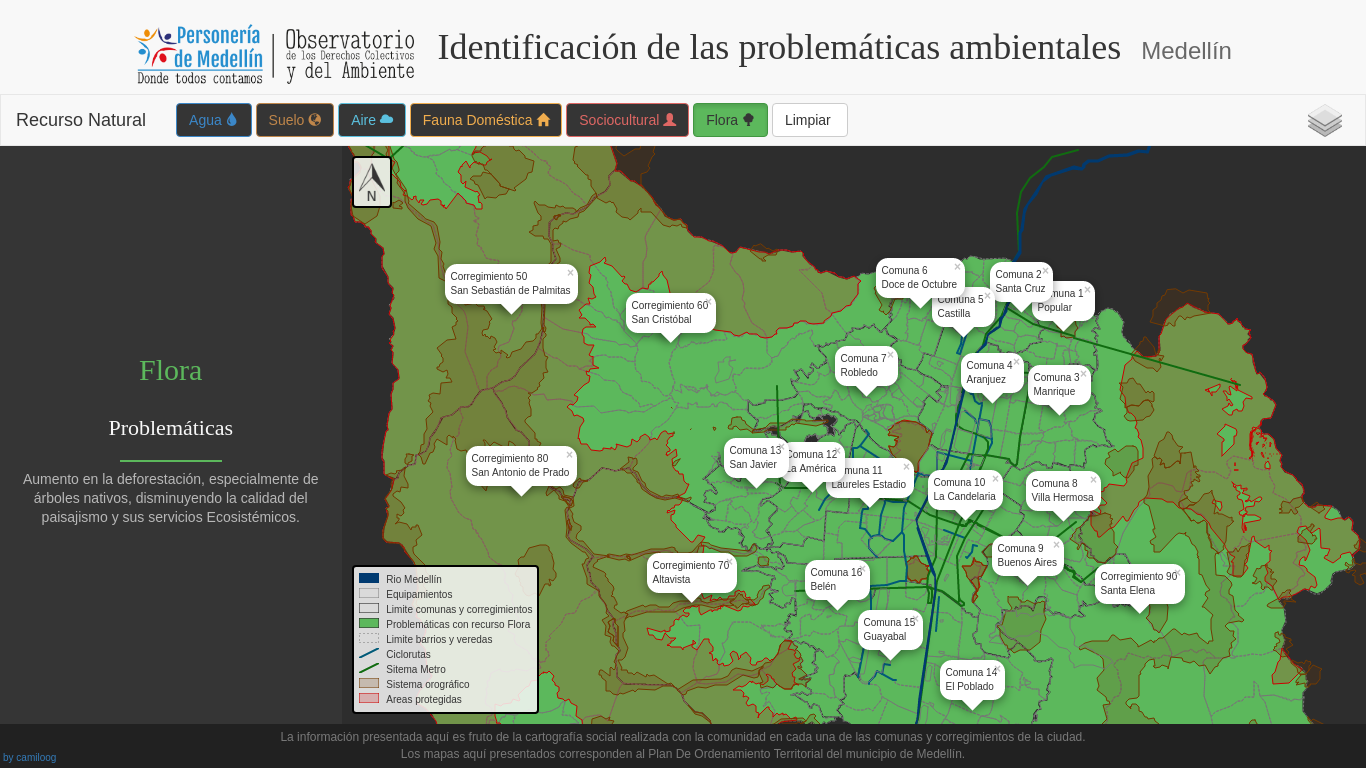
\includegraphics[width=\textwidth]{../assets/images/recurso_natural/recurso_flora.png}
	\caption{Flora}\label{fig:rFlora}
\end{subfigure}
\caption{Impresiónes de pantalla del aplicativo correspondentes a las problemáticas de cada recurso natural. Estas imágenes pueden ser encontradas en {\tt assets/images/recurso\_natural/}.}\label{fig:recurso}
\end{figure}


\newpage
\bibliographystyle{unsrt}
\bibliography{references}

\end{document}